%\documentclass[12pt,oneside,a4paper,doublespacing]{article} % for submission
\documentclass[11pt,oneside,a4paper]{article} % for sharing

\usepackage{appendix}
\usepackage{amsmath}
\usepackage{caption}
\usepackage{placeins}
\usepackage{graphicx}
\usepackage{subcaption}
%\usepackage{subfig}
\usepackage{longtable}
\usepackage{setspace}
%\usepackage{tikz}
\usepackage{booktabs}
\usepackage{tabularx}
\usepackage{xcolor,colortbl}
\usepackage{chngpage}
%\usepackage[active,tightpage]{preview}
\usepackage{natbib}
\bibpunct{(}{)}{,}{a}{}{;} 
\usepackage{url}
\usepackage{nth}
\usepackage{authblk}
\usepackage[most]{tcolorbox}
%\usepackage{xcolor}
\usepackage[usenames, dvipsnames]{color}
%\usepackage{hyperref}
%\usepackage{color}
%\usepackage{fontspec}
%\usepackage{pdfsync}
\usepackage[normalem]{ulem}
\usepackage{amsfonts}
\usepackage{xfrac}
%\renewcommand{\listtablename}{List of Appendix Tables}
%\newcolumntype{C}[1]{>{\centering\let\newline\\\arraybackslash\hspace{0pt}}m{#1}}
%\newcolumntype{L}[1]{>{\raggedright\let\newline\\\arraybackslash\hspace{0pt}}m{#1}}
% working on this need to concatenate file name based on sex and variable name
%\newcommand\Cell[1]{{\raisebox{-0.05in}{\includegraphics[height=.2in,width=.2in]{Figures/ColorCodes/\expandafter#1}}}}  

%%%%%%%%%%%%%%%%%%%%%%%%%%%%%%%%%%%%%%%%%%%%%%%%%%%%%%%%%%%%%%%%%%%%%%%%%%%%%
% setting color to letters affects spacing. Here's a hack I found here:
% http://tex.stackexchange.com/questions/212736/change-letter-colour-without-losing-letter-spacing
%\DeclareRobustCommand{\spacedallcaps}[1]{\MakeUppercase{\textsc{#1}}} % all
% caps with better spacing

%\colorlet{RED}{red}
%\colorlet{BLUE}{b}
%\colorlet{rd}{red}
%\colorlet{bl}{blue}

%%%%%%%%%%%%%%%%%%%%%%%%%%%%%%%%%%%%%%%%%%%%%%%%%%%%%%%%%%%%%%%%%%%%%%%%%%%%%%

\newcommand\ackn[1]{%
  \begingroup
  \renewcommand\thefootnote{}\footnote{#1}%
  \addtocounter{footnote}{-1}%
  \endgroup
}
%\newcommand\vt[1]{\textcolor{rd}{#1}}
%\newcommand\eg[1]{\textcolor{bl}{#1}}

%\newcommand\tg[1]{\includegraphics[scale=.5]{Figures/triadtable/triad#1.pdf}}
%\newcommand\tgh[1]{\raisebox{-.25\height}{\includegraphics[scale=.3]{Figures/triadtable/triad#1.pdf}}}

\defcitealias{HMD}{HMD}
\newcommand{\dd}{\; \mathrm{d}}
\newcommand{\tc}{\quad\quad\text{,}}
\newcommand{\tp}{\quad\quad\text{.}}
% junk for longtable caption
\AtBeginEnvironment{longtable}{\linespread{1}\selectfont}
\setlength{\LTcapwidth}{\linewidth}

%%%%%%%%%%%%%%%%%%%%%%%%%%%%%%%
\begin{document}

\title{Healthy life expectancy, mortality, and age prevalence of morbidity}

\author[1]{Tim Riffe}
\author[1]{Alyson van Raalte}
\author[1]{Maarten J. Bijlsma}
\affil[1]{Max Planck Institute for Demographic Research}

%\author{[Authors]}

\maketitle

\begin{abstract}
In calculating period healthy life expectancy, the use of age-specific morbidity
prevalence patterns assumes that age captures the important
time-variation in the given health condition, i.e.
that the disabling process is related to how long an individual has lived.
However, many common disabling processes are better measured by a time-to-death
pattern. At advanced ages the conflation of an increasing chronological-age
mortality pattern and a time-to-death morbidity pattern produces an apparent morbidity pattern that also increases with advancing age. Differences in period healthy life expectancy over time or between populations
cannot easily be partitioned into morbidity and mortality components because
the period morbidity pattern may depend on an unknown future time-to-death
process not captured by period mortality. We illustrate these
concepts formally and empirically, using morbidity data from the U.S. Health and Retirement Study. While holding
the time-to-death morbidity pattern fixed, we show that mortality reduction
alone reduces the total life years with disability. We estimate the magnitude of this bias for different disabling processes. This has implications for any between- or within-population comparisons of period healthy life expectancy conditioned on different age patterns of mortality.
\end{abstract}

\section{Introduction}

Healthy life expectancy (HLE) is among the most widely used metrics of
population health. It combines information on mortality and morbidity to summarize the expected years of life lived in good health, however measured. If healthy life expectancy increases faster than life expectancy, morbidity is compressed into a smaller proportion of life. HLE can increase because of changes mortality, morbidity, or both.

In calculating HLE, the use of age-specific morbidity prevalence data implicitly
assumes that a chronological age pattern best characterizes variation in the
health characteristic over the lifespan.
However, \citet{riffe2015ttd} show that many common disabling
processes are better measured by a pattern over time-to-death (TTD) or by both age and TTD. Most morbidity
patterns increase with age, and can claim empirical regularity in this regard.
However, we explain how the observed shape of a morbidity age-curve can change
due to changes in mortality even with no underlying change in morbidity. At advanced ages the conflation of an increasing chronological-age
mortality pattern and a TTD morbidity pattern produces an apparent morbidity pattern that also increases with advancing age. 

In the
cohort perspective the true and apparent morbidity patterns imply the same HLE.
Problems arise in the period perspective. Differences in period HLE over
time or between two populations cannot easily be partitioned into morbidity and
mortality components, because the period morbidity component will depend on some unknown future TTD process. For the same reason, comparisons of disability prevalence rates by age are not recommended between populations with different underlying age schedules of mortality.

In this paper we illustrate these concepts formally and empirically, using
morbidity data from the U.S. Health and Retirement Study \citep{HRS}. While
assuming a fixed TTD morbidity function, we show that mortality
reduction alone can reduce the total life years with disability (DLY). We
estimate the magnitude of potential biases for different disabling processes,
given different levels of mortality extracted from the Human Mortality Database
\citep{HMD2015}. We first explain how the age pattern of morbidity may partly be
a function of mortality using both formulas and a schematic illustration.


\section{Morbidity as a function of time-to-death}
 
Imagine a bad health condition, $G$, with prevalence that varies as a
function of time-to-death, $y$, and not as a function of chronological age, $a$.
Since the TTD prevalence distribution in older ages is something
close to exponential, there will still be an apparent age function,
$g^\star(a)$.
In this case $g^\star(a)$ is a heterogeneous aggregate based on both mortality
and the underlying TTD process:
 
\begin{align}
g^\star(a) &= \frac{\int _0^\omega g(y) N(a,y) \dd y}{N(a)} \\
      &= \frac{\int _0^\omega g(y) N(a)
      \mu(a+y)\frac{\ell(a+y)}{\ell(a)}\dd y}{N(a)}\\
      &= \int _0^\omega g(y) f(y|a)\dd y \label{eq:gyfya}\tc
\end{align}
where $N(a)$ is the population aged $a$, $\ell(a)$ is lifetable survivorship, and
$\mu(a)$ is the force of mortality. $f(y|a)$ is the conditional remaining-years
distribution, which gives the probability of dying in $y$ years given survival
to age $a$. The expression \eqref{eq:gyfya} says that the proportion of those in
age $a$ that has condition $G$ does not depend on population structure at all, but only on future mortality rates and the TTD pattern of $G$, $g(y)$. 

A function such as $g(y)$ would have implications for the interpretation of
period age patterns of morbidity, and by extension, HLE. If a function such as $g(y)$ holds, it is tautologically true that the
measurement of HLE in completed cohorts (or stationary populations)
will be identical whether calculated on the basis of $g^\star(a)$ or the
underlying $g(y)$ pattern. Distortions only arise in the interpretation of
period HLE under changing mortality, or with period HLE comparisons between
populations with different mortality. 

%Under changing mortality and a fixed $g(y)$, the age pattern of
%morbidity, $g^\star(a)$, will change even as the morbidity process does not,
% and this is why 

Since morbidity prevalence in this scenario is partly a function of mortality,
 the age patterns of morbidity for populations with different mortality
levels or patterns cannot be compared without additional information. Under
these circumstances, it is also deceptively tricky to partition period HLE
differences into underlying morbidity and mortality components, because the
morbidity component is (arithmetically) a function of an uncertain future mortality pattern
that accompanies the apparent age pattern of morbidity. Although cohort HLE (a
gold standard) is theoretically unbiased \citep{imai2007estimation}\footnote{We confirm that this remains so even if morbidity prevalence in strongly patterned by time-to-death.}, and therefore comparable, this quantity cannot be faithfully
decomposed into morbidity and mortality components based on age patterns of morbidity and mortality alone if
the underlying morbidity pattern is a function of time-to-death.

A toy example serves to illustrate these concepts. Figure~\ref{fig:test}
provides a schematic overview of two stationary populations. The
underlying survival pattern of these two populations is based on period survival
curves from Japanese males in 1970 (a) and 2010 (b) (HMD), but the reader may
imagine these as two hypothetical populations. Population (a) has a life
expectancy of 69.3, while population (b) has a life expectancy of 79.5, slightly
more than 10 years higher. For demonstration, we partition each survival curve
into 10 lifespan quantiles, represented with horizontal bars. Our simple
TTD prevalence, $g(y)$, is drawn with identical yellow triangles at
the end of each lifespan bar. Onset begins 5 years before death and culminates with 80\%
prevalence. The chronolgical prevalence function is drawn with blue triangles,
with onset at age 50 reaching a maximum prevalence of 50\% at hypothetical age
111.5. Both prevalence functions are identical for populations (a) and (b). 

\begin{figure}
\centering
\begin{subfigure}{.5\textwidth}
  \centering
  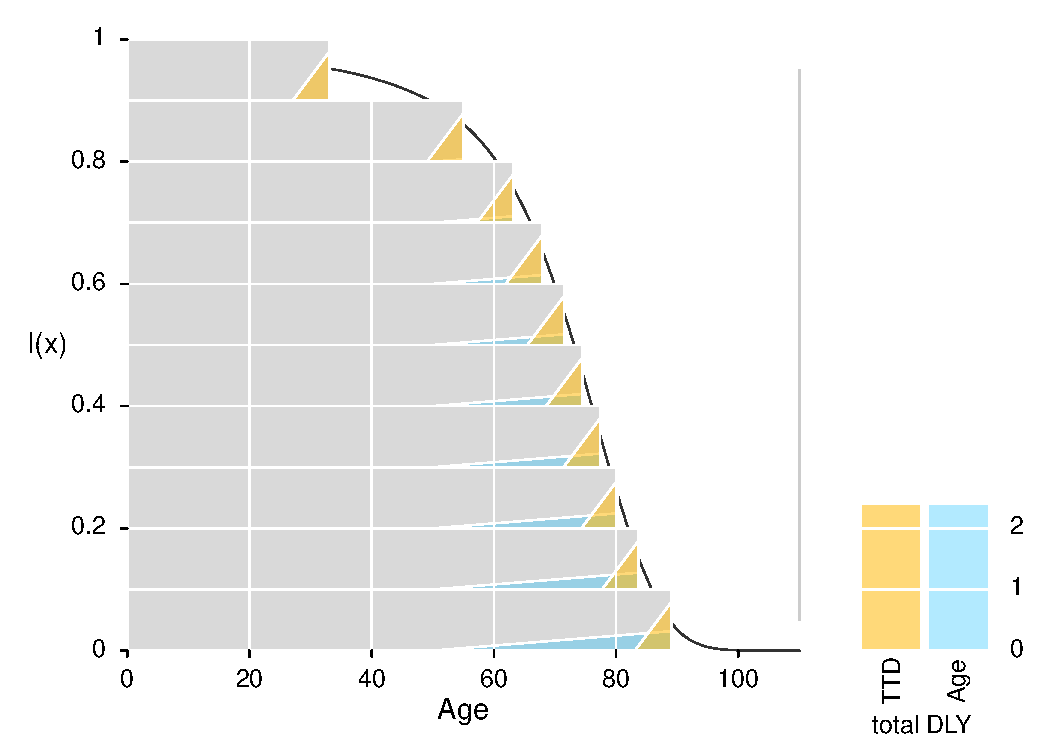
\includegraphics[width=.98\linewidth]{Figures/Japan1970}
  \caption{Higher mortality setting}
  \label{fig:toypop1}
\end{subfigure}%
\begin{subfigure}{.5\textwidth}
  \centering
  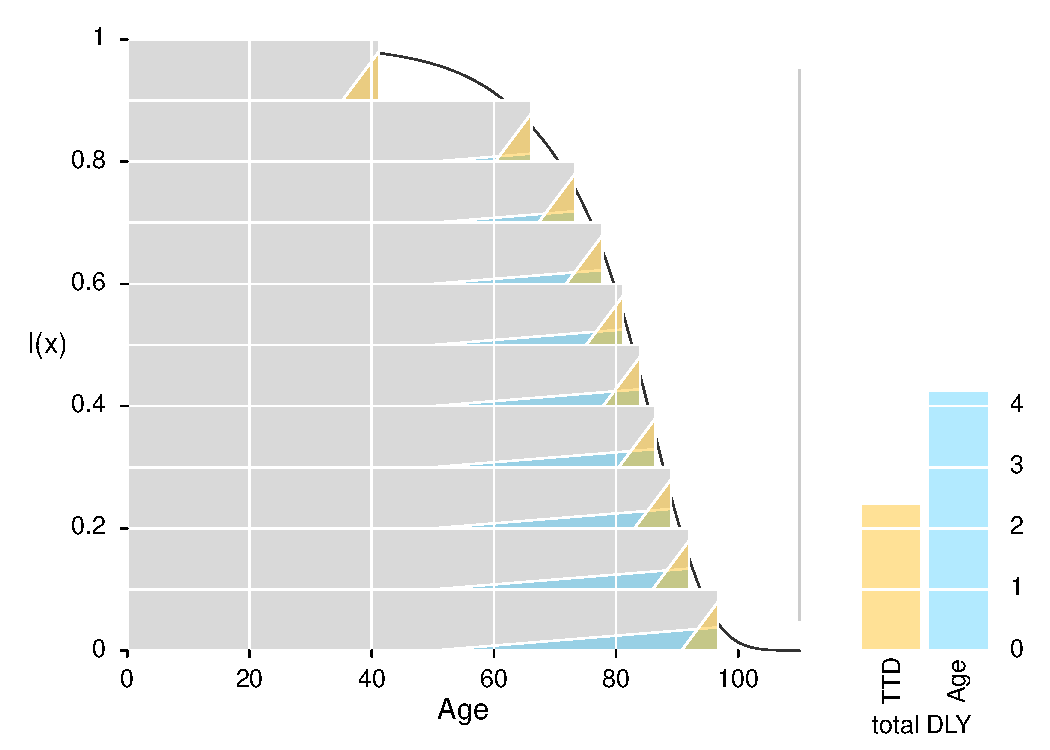
\includegraphics[width=.98\linewidth]{Figures/Japan2010}
  \caption{Lower mortality setting}
  \label{fig:toypop2}
\end{subfigure}
\caption{Schematic survival curves from higher (\ref{fig:toypop1}) and lower
(\ref{fig:toypop2}) mortality populations. Each population is
subjected to the same chronological age (blue) and time-to-death (yellow)
morbidity prevalence patterns. The total prevalence of each sums to disability life years
(DLY), drawn on the right of each survival curve. In \ref{fig:toypop1}
the age and time-to-death prevalences imply the same DLY. In
\ref{fig:toypop2} the time-to-death DLY is identical to \ref{fig:toypop1}, but
the age DLY is two years higher, due entirely to improved longevity.}
\label{fig:test}
\end{figure}

The resulting disability life years (DLY) is shown with
barplots next to each stationary population.
In population (a) the age and TTD prevalence functions yield
the same DLY (and HLE). In population (b) the time-to-death DLY is identical to
population (a), but the age DLY is nearly twice as high. For the
age prevalence function, it is correct to conclude that increased longevity leads to
increases in prevalence, but for the TTD prevalence function there is
no morbidity-mortality trade-off. Instead, improved longevity leads to increased proportions of life
lived disability-free, albeit with no change in the absolute concentration of morbidity in the final years of life. Analyses
based on the standard Sullivan method \citep{Sullivan1970} are only capable of
predicting increased DLY when projecting from the mortality of (a) to (b). This
is so for both kinds of morbidity because the TTD prevalence pattern
is erased when the same condition is measured over age. The same
Sullivan method can also only conclude that the morbidity of the TTD
process is more compressed in (b) than in (a), even though its essential
character is unchanged. Prevalence functions are in fact more nuanced than those
presented here, but our example provides a useful heuristic to understand a previously-undescribed source of bias in common applications of the Sullivan method.

\FloatBarrier
\section{How changing mortality affects morbidity prevalence}

The age pattern of morbidity prevalence observed in the cross-section (in older ages) depends
on the extent to which prevalence is principally described by
age versus TTD and on the underlying mortality
level. If the prevalence is principally a function of TTD, the
specifics of its shape are also important. In Figure~\ref{fig:Fig_schematic3} we
show the age-translations of different TTD prevalence patterns when
interacted with fictitious stationary populations under different mortality levels.

\begin{figure}
\begin{adjustwidth}{-1.5cm}{}
	\centering
	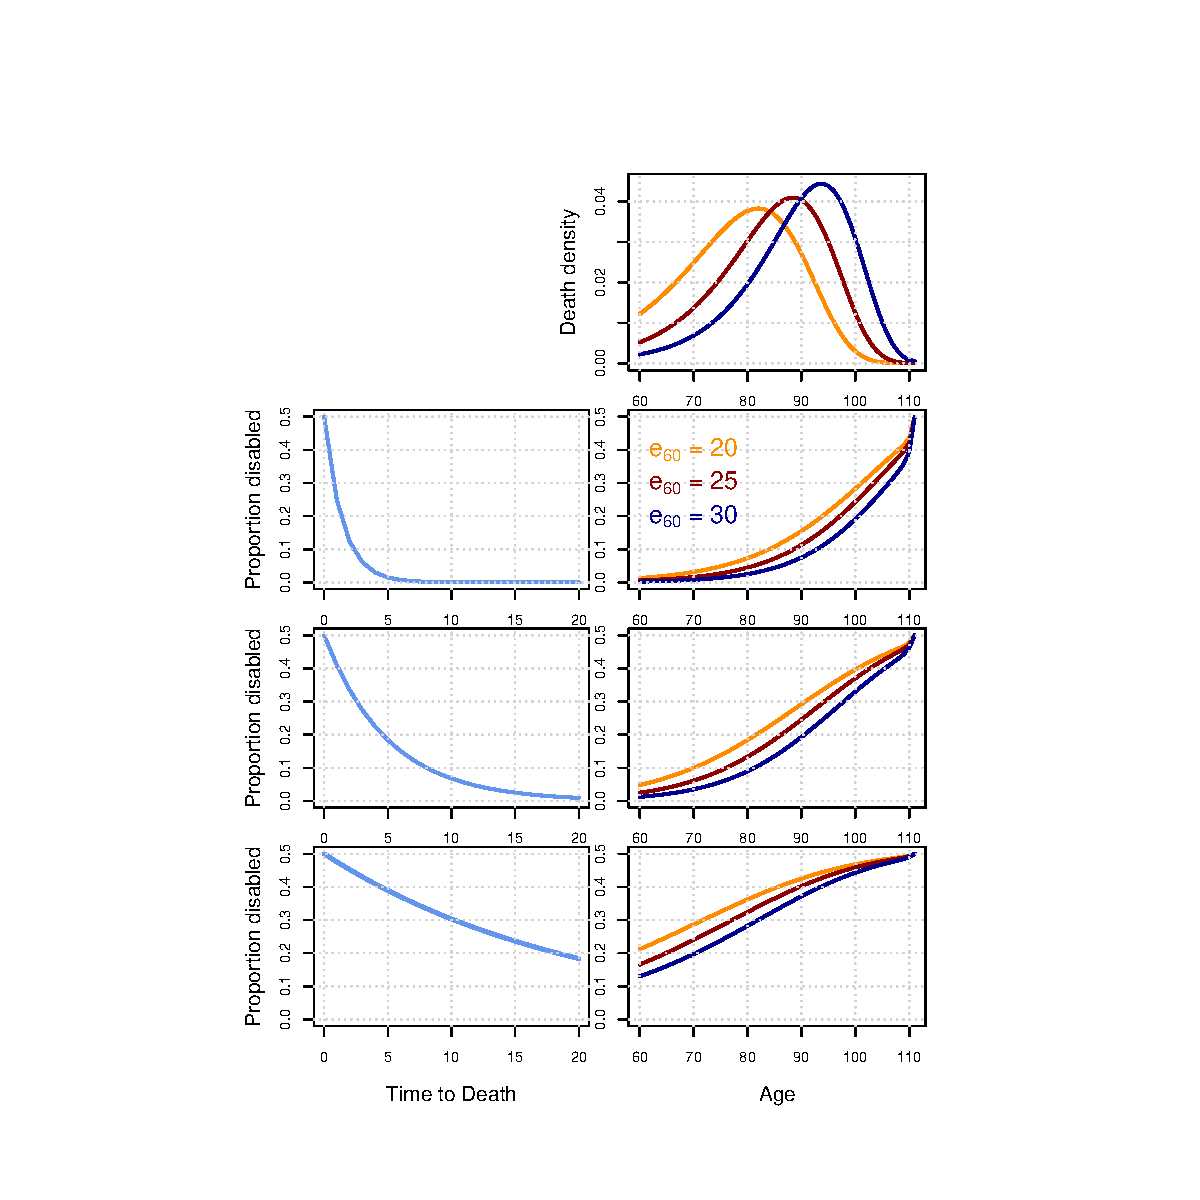
\includegraphics[scale=.8]{Figures/schematic3.pdf}
	\caption{The age pattern of morbidity prevalence in ages 60$+$ derived from interacting different TTD prevalence patterns (left column) with fictitious stationary populations subject to the color-coded death distributinos depicted in the top right figure.}
	\label{fig:Fig_schematic3}
\end{adjustwidth}
\end{figure}

The first column contains three different types of disability, all of which are
experienced by half of the population at the time of death, but which differ in
the timing of onset prior to death and in the steepness of the curve with the
approach to death.
The first type of disability is virtually nonexistent 5 years prior to death, but then increases very rapidly as death approaches. The middle variant of disability is rare 15 years before death, but increases to about 20 percent of the population 5 years before death and rises sharply thereafter. The bottom figure depicts a disabling process that although still strictly determined by time-to-death, is common and accumulates very slowly starting from about 50 years before death.

The second column translates the time-to-death disability prevalence curves into
the ``apparent'' chronological age prevalence of disability for different
mortality levels depicted by the death density curves above. These mortality
levels roughly correspond to USA males in 2002 $e_{60} = 20.0$ years, Canadian
females in 2004 $e_{60} = 25.0$ years, and projected Japanese females a decade
or so from now $e_{60} = 30.0$ years (latest observed level in 2012 was $e_{60}
= 28.3$ years \citep{HMD2015}). In all cases increasing remaining life
expectancy results in decreasing age-specific disability prevalence by
chronological age. With steeply increasing disability prior to death (first
row), the differences in disability prevalence are largest above age 80, where
the bulk of mortality occurs, while with more gently increasing disability
(second and third rows) the greatest differences in disability age-prevalence
curves appear at younger ages.

These differences induced by mortality alone are not trivial. In the middle variant, which closely resembles the TTD prevalence of disability in bathing, a 10-year increase in $e_{60}$ results in a 50 percent drop in disability prevalence at age 80 from around 20 to 10 percent. Meanwhile, the age at which a quarter of the population were considered disabled in this scenario differed by about 5 years with a 5-year improvement in $e_{60}$ from 20 to 25.

Of course the disability prevalence is rarely a function of thanatological age
alone. For example, Figure~\ref{fig:IADL_ATL} shows US male
IADL-disability prevalence broken down by age and TTD.
The horizontally running gradients indicate that time-to-death is a more important time axis to predict deterioration in IADL than
time since birth. Thus our assumption of fixed morbidity prevalence on the
time-to-death axis is not unrealistic, at least for some characteristics. This
is the case for many, but not all, indicators of health and disability \citep{riffe2015ttd}. In
reality, the prevalence of disability varies on both the age and
time-to-death axes. The degree to which prevalence is better measured by age or
time-to-death for different disabling conditions remains an open research
question.

\begin{figure}
\begin{adjustwidth}{-1.5cm}{}
	\centering
	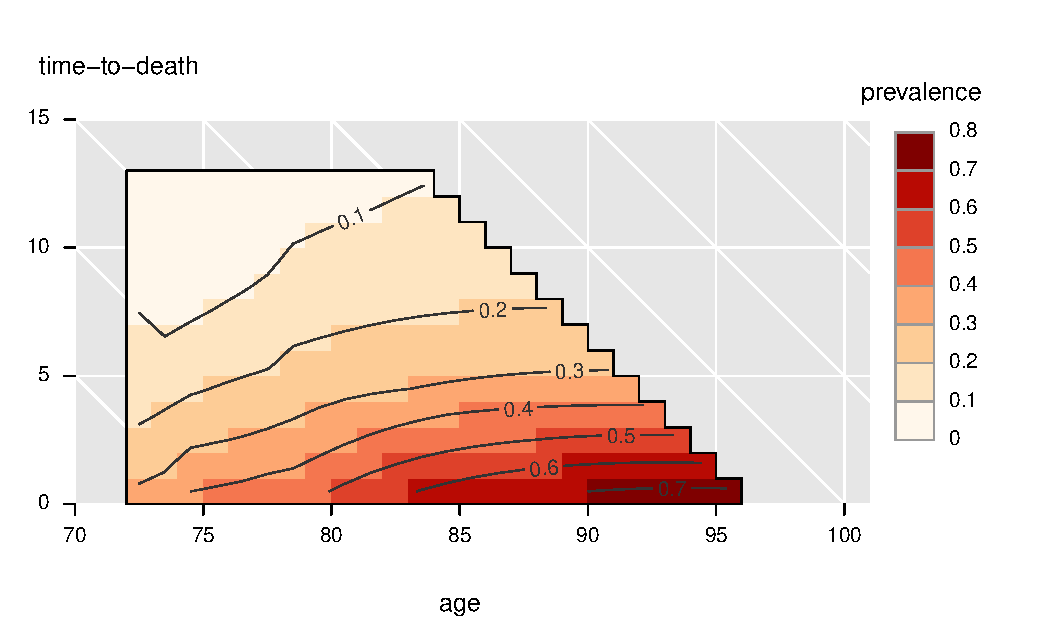
\includegraphics[scale=.8]{Figures/IADL1_Males.pdf}
	\caption{Proportion of males from the 1915-1919 cohort with at least one (of
	five) instrumental activity disabilities, by time-to-death and age.}
	\label{fig:IADL_ATL}
\end{adjustwidth}
\end{figure}


\FloatBarrier
\section{Estimating bounds for the impact of mortality differences on estimates of disabled life years}

The Sullivan method is the most commonly used method to partition life
expectancy into estimates of the total life years lived in a state of good
health (HLY) or disability (DLY). Its popularity owes to its minimal data
requirements. Only current age-specific disability prevalence rates are needed
in addition to a life table or age-specific mortality rates. Specifcally, the
number of person-years with disability $_{n}\pi _{x} \cdot _{n}L _{x}$ in
age-group $x$ to $x+n$ are the product of the person-years lived from the life
table $_{n}L _{x}$ and the proportion disabled $_{n}\pi _{x}$. The total DLY is
the sum of  $_{n}\pi _{x} \cdot _{n}L _{x}$ over all age groups
\citep{Sullivan1970}.

It has long been recognized that the Sullivan method does not produce a pure
synthetic measure of health expectancy, since it combines flow data of current
mortality incidence with stock data of morbidity prevalence. While the mortality
flow responds immediately to period change, for instance from medical
innovations, the morbidity stock is slower to change because it reflects past
cohort experiences with disability incidence and recovery
\citep{Mathers1997,Barendregt1994}. Moreover, as was illustrated in
Figure~\ref{fig:Fig_schematic3}, the prevalence at any age may not only depend
(mathematically)) on past transitions into and out of disability but also on
future deaths.

Nevertheless, comparing populations on the basis of life years lived in a state
of good health (HLE) or disability (DLY) is standard practice in population
health. The difference in either metric, either a within-population difference
over two time periods or a between-population difference in the same time
period, is often decomposed into mortality and morbidity components on the basis
of differences in survivorship and morbidity age-prevalence respectively
\citep{Nusselder2004,Andreev2002}. According to \citet{Nusselder2004}, the corresponding mortality and disability effects at each age group for a within-population decomposition are:

\begin{align}
	{_{n}{MOR}_{x}}&=\left [ \frac{_{n}\pi_{x\left ( t \right )} + _{n}\pi_{x\left
	( t+y \right )}  }{2}\right ]\cdot \Delta _{n}L_{x} \label{eq:MORcomp}\\
	{_{n}{DIS}_{x}}&=\left [ \frac{_{n}L_{x\left ( t \right )} + _{n}L_{x\left (
	t+y \right )}  }{2}\right ]\cdot \Delta _{n}\pi_{x}	\tc \label{eq:DIScomp}
\end{align}
where $\Delta$ refers to the change in the variable from time $t$ to $t+y$,
$_{n}\pi_x$ is prevalence in the discrete age group $[x,x+n)$, and $L_x$ is
lifetable exposure. Discrete prevalence $_{n}\pi_x$ is essentially our
$g^\star(a)$ from equation~\eqref{eq:gyfya}. The sum of the two components over
all ages is equal to the total change in DLY. These formulas are essentially an
application of standard \citet{kitagawa1955components} decomposition.

Although it is true that these two components arise from changes in survivorship
and morbidity prevalence respectively, difficulties arise in the interpretation
of the components as pure mortality and disability effects. If the time-to-death
profile of disability prevalence does not change over different mortality
regimes, inducing mortality decline alone will result in declines in the
age-pattern of prevalence component, as we demonstrated. This method of
decomposition will therefore still attribute a portion of the
change in DLY to morbidity, and we consider this to be a source of bias.

To get a sense of the upper magnitude of this bias, we test how the disability
component of this decomposition method would change when a fixed time-to-death
prevalence of morbidity is applied to different mortality regimes using empirical data. Morbidity data come from the US Health and Retirement Study while mortality and exposure data come from the Human Mortality Database \citep{HMD2015}.

Specifically, we consider the age prevalence of difficulties in carrying out at
least 1, 2, or 3 (out of 5) functional Activities of Daily Living (ADL),
difficulties in carrying out at least 1, 2, or 3 (out of 5) instrumental
Activities of Daily Living (IADL), living in a nursing home, having poor
self-rated health, and being unable to name the month of the year. We estimate
these time-to-death prevalences for quinquennial cohorts from 1905 to 1930,
separately for males and females. We calculate the time-to-death $g(y)$ profiles of
disability prevalence for all extinct lifespans above age 65 for each cohort.
Estimation is done via a loess smooth over age, time-to-death, and birth
cohorts. We
then average the time-to-death profiles of disability over lifespans and over the 6 cohorts.
% TR: no mort assumptions needed to blend thano profiles, as these are in
% principle purged of mortality.
% For more
%recent cohorts, we forecasted morbidity and mortality rates to close the cohort
%out at age 110. This was generally a small proportion of the total cohort, for
%instance from the 1915 birth cohort 6 percent of males and 11 percent of
% females were still alive. 
 The time-to-death prevalence of morbidity for
each disability type is shown for females in Figure~\ref{fig:DisbyTTD}.


\begin{figure}
\begin{adjustwidth}{-1.5cm}{}
	\centering
	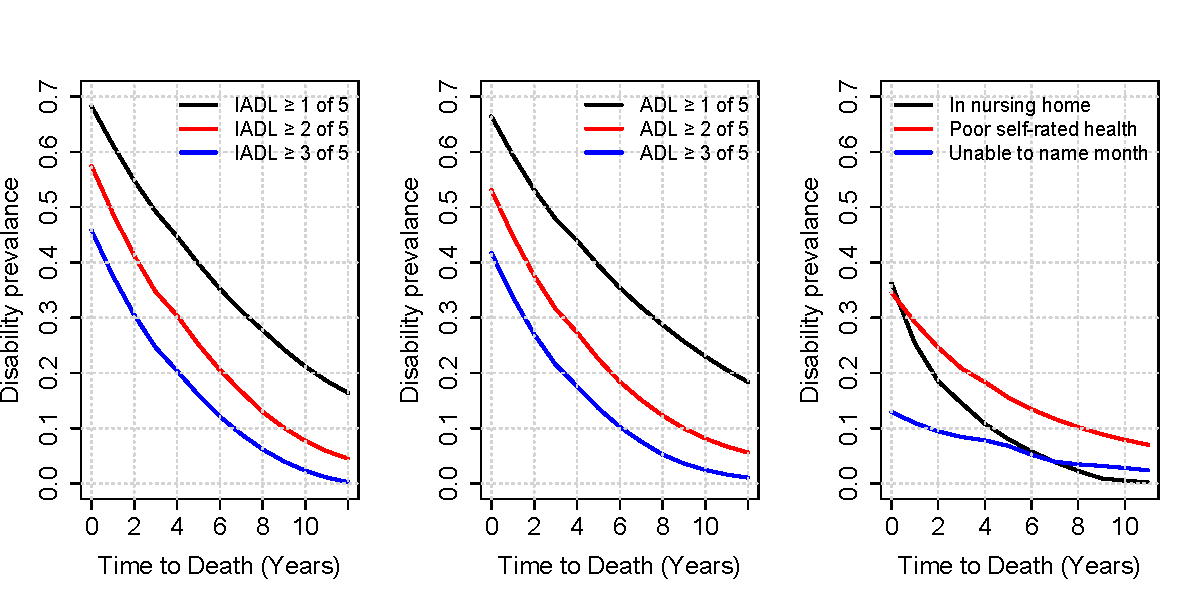
\includegraphics[scale=.6]{Figures/DisbyTTD.pdf}
	\caption{The disability prevalence by time to death for various disability types, based on American HRS data (females).}
	\label{fig:DisbyTTD}
\end{adjustwidth}
\end{figure}


We calculate the apparent period chronological age prevalence of morbidity,
$g^\star(a)$, for all medium to large populations of the Human Mortality
Database, had they experienced the US time-to-death profile of morbidity. Eastern European countries are excluded from this exercise due to widely varying
age patterns of mortality, particularly in the years surrounding political
transition. To calculate the age-pattern of morbidity, we assume the survival
pattern of each lifetable to be a stationary population and apply a
discretization of equation~\eqref{eq:gyfya}. 

We then make pair-wise comparisons of DLY between each population in
the same year for the years 1980, 1990, and 2000.
For within-country comparisons, we compare each population in
10-year jumps, for all years starting from 1950. Altogether this leads to
187 within-population comparisons and 1785 between-population comparisons for
each sex. Finally we decompose the change or difference in DLY between the
population pairs into mortality and morbidity components using the
\citet{Nusselder2004} method described above and in
Equations~\eqref{eq:MORcomp} and \eqref{eq:DIScomp}. The
true value of the change in DLY and the true value of the disability component
are both zero by design. Thus, the estimated disability component from this
decomposition gives a gauge of bias.

We compare the association between the change in the disability component
(Equation \ref{eq:DIScomp}) and the increase or difference in remaining life
expectancy at age 60 for each population pair in
Figure~\ref{fig:Fig_Decomp_3x3}. By doing so we aim to provide a rough
empirically-based estimate of the upper bound of the change in the disability
component that is attributable to the different underlying mortality levels
of any two populations being compared. Thus if female $e_{60}$ increases in a
country by 5 years, up to about 1 year of the reduction in DLY that is
attributed to the disability component could be solely arising from the decrease
in mortality, in the case where disability is measured as having difficulty in
at least three ADLs. Departure from this upper bound in real life depends on
the degree to which the disability prevalence changes on a time-to-death versus chronological
age axis, the extent to which the US average time-to-death prevalence is
representative, and the departure from the stationary population assumption.

Overall, the relationship between the change in disability component and the
increase in $e_{60}$ is strikingly linear although the slopes differ for males
and females and by disability type. To some extent this is because the
final level of disability prevalence (i.e. in the final year of life) differs by
disability type.
In Appendix Figure~\ref{fig:Fig_Decomp_3x3_rel} we standardize for the maximum
disability prevalence to give a clearer comparison between disability types.
Even after standardization, the change in the disability component is
greater with larger $e_{60}$ differences for disability types with more
gradually changing prevalence levels by time-to-death and for females who
likewise have more gradually changing prevalence levels by time-to-death.
This is because steep time-to-death profiles of disability concentrate
disability prevalence near the death distribution,
whereas gradually changing (but still entirely time-to-death) disability
profiles spread out disability prevalence over a wider range of ages before
each age at death.

\begin{figure}
\begin{adjustwidth}{-1.5cm}{}
	\centering
	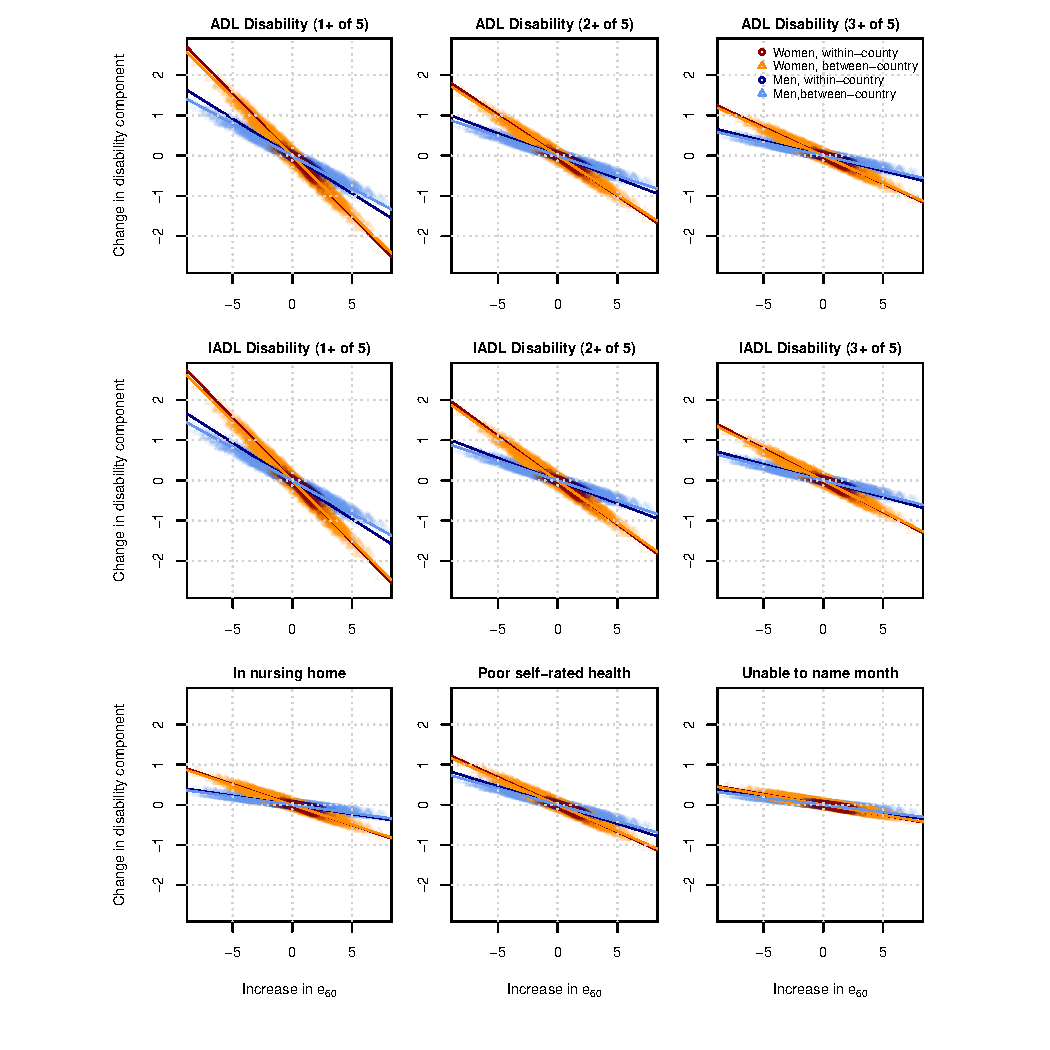
\includegraphics[scale=.8]{Figures/Decomp_3x3.pdf}
	\caption{Results of the hypothetical decomposition exercise. The size of the
	morbidity component using a standard decompositon method is plotted against
	the difference in remaining life expectancy at age 60 ($e_{60}$) in each
	pair of populations. Linear trend lines are also provided for each sex and decomposition type.}
	\label{fig:Fig_Decomp_3x3}
\end{adjustwidth}
\end{figure}

If projecting morbidity prevalence, one can also refer to these results as a
heuristic on the bias inherent in assuming a fixed age-pattern of morbidity.

\FloatBarrier
\section{Discussion}

Healthy life expectancy remains a popular tool for analyzing population health.
At any given time, a snapshot of the life years lived in good or poor health is
captured. This information is well-summarized in both the period and
cohort perspective, regardless of whether morbidity prevalence is a function of
chronological age or time until death. Difficulties arise in the
interpretation of period differences in this quantity. The chronological age
pattern of disability can increase or decrease solely as a function of mortality
change even when the underlying morbidity function is held constant. Thus, for
instance, observed widening ratios in the age profiles of disability prevalence
between subgroups \citep{Crimmins2001} cannot be attributed to changes in the
disabling process without taking into account changing mortality profiles. This
observation calls into question the practice of forecasting observed
age-specific rates of decline in disability \citep{Manton2006,Khaw1999}, and
especially the more common practice of holding age-patterns of disability fixed
in morbidity projections.
Health economists refer to a similar `red herring' argument, namely that medical costs are more closely associated with time-to-death than with chronological age. As a result, health
care cost projections based on a chronological age rather than time-to-death
pattern of expenditure are artificially inflated \citep{Zweifel1999,Geue2014}.

Instead, we argue that the better way to measure changes in health or disability
is from a cohort perspective \citep{Manton2000,Manton2008,Christensen2013}.
\citet{Manton2000}, for instance, found large differences between period and
cohort estimates of active life expectancy (ALE). ALE at ages 65 and 85 was
between 1.6 and 2.6 times larger in the cohort perspective than for similar
period estimates, and the expected years of life disabled were smaller in the
cohort perspective.
Additionally, they uncovered larger differences between the cohort and period
perspectives for men than women, which they attribute to differences in
disability transition rates between the sexes. We hypothesize that some of these
larger differences might also be attributable to larger mortality reduction
among men. Further, while cohort HLE estimates are unproblematic as an index,
decompositions of HLE differencs between cohorts into morbidity and
mortality components are usually biased. This is because the age pattern of
morbidity is itself decomposable into morbidity and
mortality components, as we demonstrate.  

Several studies have looked at the macro relationship between overall mortality
levels and sex differences in HLE. At higher levels of life expectancy, female
advantage in healthy life expectancy diminishes, or even reverses into male
advantage \citep{vanOyen2013}. Meanwhile, the larger the proportional female
advantage in longevity, the larger the female excess in the proportion of life
in poor health \citep{Luy2014}. That mortality levels and disability prevalence
are related is perhaps not surprising. As our example illustrates, differences
in underlying mortality can lead to differences in the age profile of
disability.
Additionally, although the association between the severity of chronic conditions and poor health was found
to be similar for men and women, morbidity prevalence rates are generally higher
among women, particularly for arthritis and chronic pain \citep{Case2005}. It
would be worthwhile to investigate whether there might not only be differences
in the composition of chronic conditions between the sexes, but whether the
underlying morbidity process itself might differ between the sexes in its
chronological versus time-to-death axis \citep{riffe2015ttd}.

In reality, not all end-of-life health conditions are exclusive functions of
time-to-death, but morbidity often varies as a function of
both aspects of time, and expressing morbidity prevalence
as a function of both age and time-to-death, $g(a,y)$, can increase precision
\citep{wolf2015disability,riffe2015ttd}.
There is great variety in the temporal variation of the prevalence of late-life
health conditions. There is also great variety in individual trajectories with
the approach to death \citep{lunney2003patterns}. That morbidity prevalence may for certain health conditions be a function of
time to death does not imply that morbidity incidence is necessarily a function
of time to death. First, an age-patterned sequence of health states wherein
mortality risk increases with passing states could produce a time-to-death
prevalence pattern, \textcolor{red}{e.g. an accumulation of DNA damage over time
resulting in increased ristks of cancer and thereby death}. Second, it is also
plausible that some morbidity conditions are linked to a more general process of dying, thereby
linking morbidity to a process that ends with death and consequently producing a
time-to-death prevalence pattern. For example, certain conditions may manifest
themselves that are not (primary) causes of the impending death but
consequences of nearness to death caused by some other (primary) factor.
Either of these explanations does not conflict with the reality that causes must
precede effects, and that therefore death cannot cause the morbidity that precedes it \citep{lynch2015commentary}.

Increasingly, data on mortality incidence and recovery are available from
multiple waves of survey panels such as the HRS, allowing researchers to
calculate healthy life expectancy using sophisticated multistate models.
Unfortunately such data is not available in all countries, or if it is, time
trends are limited to the recent past. We are not arguing that a TTD approach
should replace multistate models when such data is available. Our aim is rather
to expose the implications of comparing healthy life expectancy from
age-structured prevalence-based models with different underlying mortality
regimes.

To model prevalence as a function of
time-to-death requires no surreal understanding of how things work, but is
rather a modelling choice \citep{wolf2015disability}. When modeling for
descriptive or exploratory purposes (as we have done to produce e.g. Figure 3),
\textcolor{red}{and possibly for projective purposes}, one can safely use
time-to-death as a predictive variable.
However, using time-to-death in models intended for causal interpretation is more hazardous; it is argued that time-to-death may function as a proxy for unobserved variables such as biomarkers for impending mortality \citep{wolf2015disability}. However, others argue that including this variable as a proxy in models will introduce omitted variable bias \citep{lynch2015commentary}. Regardless, even in the descriptive case, the reader may understand the time-to-death morbidity prevalence pattern $g(y)$ as generally hypothetical, since the current evidence base is limited in scope. Much more empirical work is needed in order to determine whether modeling morbidity
prevalence as a function of time-to-death is more widely applicable to
other health conditions, younger ages, more recent birth
cohorts, and other populations in different stages of epidemiological
transition. Further, the more nuanced function $g(a,y)$ changes over time and it
is not fixed as in our examples. Nevertheless, the distortions demonstrated are likely to arise in everyday practice when comparing health trends over age between populations and over time, since many health conditions appear to show strong time-to-death components. Trends in mortality may offset or amplify changes in morbidity.
Therefore, in order to separate effects, more careful measurements are required
than is typically the case. 

\section{Appendix}


\begin{figure}
\begin{adjustwidth}{-1.5cm}{}
	\centering
	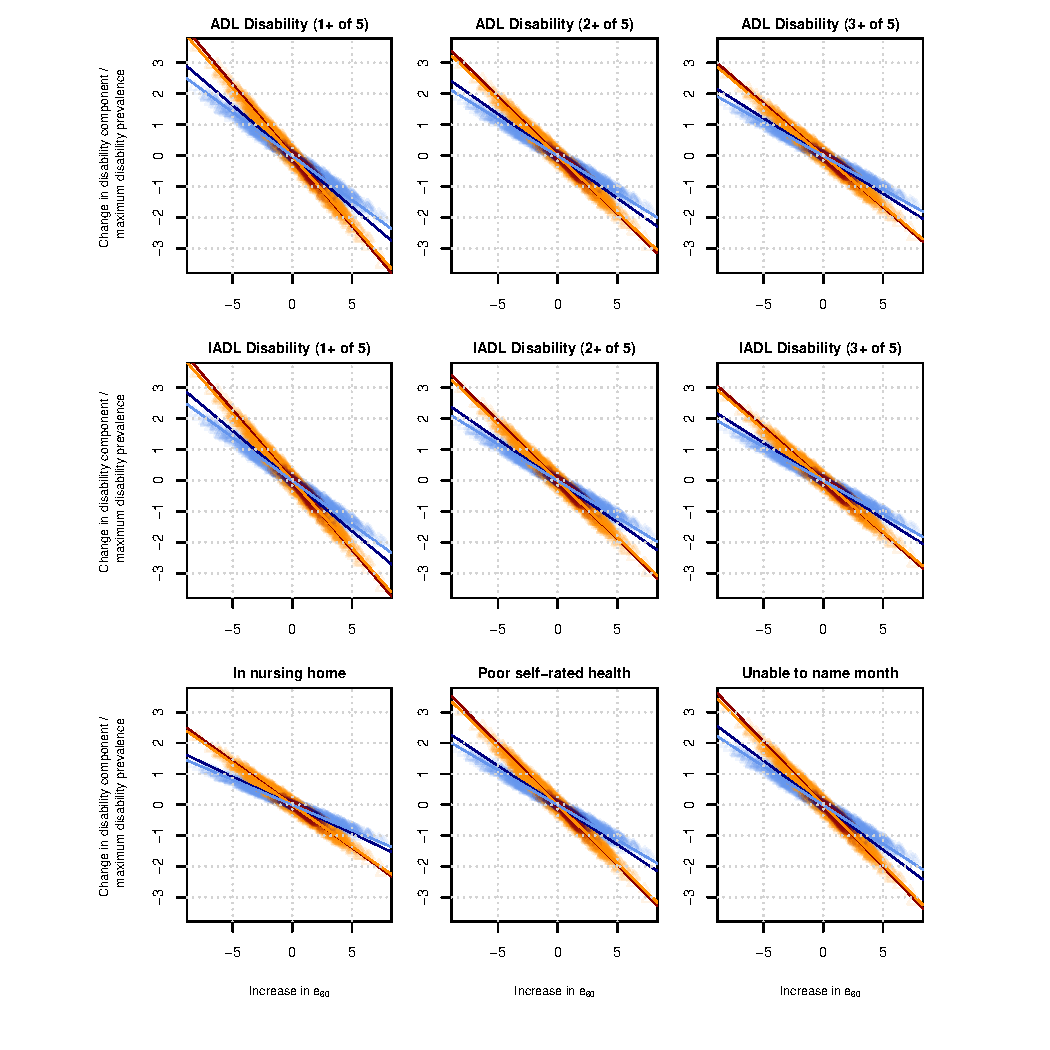
\includegraphics[scale=.8]{Figures/Decomp_3x3_rel.pdf}
	\caption{Results of the hypothetical decomposition exercise standardized to the maximum disability prevalence for each disability type. The size of the
	morbidity component using a standard decompositon method is plotted against
	the difference in remaining life expectancy at age 60 ($e_{60}$) in each
	pair of populations. Linear trend lines are also provided for each sex and decomposition type.}
	\label{fig:Fig_Decomp_3x3_rel}
\end{adjustwidth}
\end{figure}



\newpage%% this forces a new page, so that things end up a bit more where you think they should
\bibliographystyle{chicago}
\bibliography{RvRB2016refs}

\end{document}
